\startchapter{A suite of packages for scalable Whole Cell Models: WCMpy}
\label{WCMpy_chapter}

\section{Introduction}
The development of whole-cell models (WCMs) \cite{Bhat2020Whole-CellSurvey} is purported to be a defining challenge of the 21st century \cite{Tomita2001Whole-cellCentury}. WCMs amalgamate specialized models of cellular systems -- e.g. the metabolome and its kinetics rate laws; the genome and its translational units; and the proteome and its functional proteins -- into a single model that represents the entirety of a cell. This endeavor offers the unique opportunity to assess the completeness of cellular theory \cite{Palsson2000TheBiology,Feig2019Whole-cellDetail} and to answer research questions in medicine \cite{Bordbar2015PersonalizedPharmacodynamics,Loscalzo2011SystemsMedicine} and synthetic biology \cite{Purcell2013TowardsBiology}. WCMs are rooted in the Newtonian perspective that a complete model of both cellular biochemistry and environmental conditions can reproducibly recreate the phenotypes and diversity that are observed experimentally. An atomic-resolution molecular dynamics (MD) simulation of an entire cell (all $1E9$ molecules \cite[][approximated from cellular mass]{Lewis2014MassPopulations}) may be the ultimate tool to answer these audacious biological questions; however, since the state-of-the-art of MD is currently at the level of proteins \cite{Adcock2006MolecularProteins}, membranes \cite{Egberts1994MolecularMembrane,Alper1993ComputerDynamics,Alper1993TheStudy}, or small cells \cite{Perilla2015MolecularComplexes} for fractions of a second, WCMs are the available tool for simulating cellular chemistry \cite{Feig2015CompleteBiology} at biological timescales (hours to days). 

The first WCMs \cite{Karr2015TheModeling} were rudimentary systems of ordinary differential equations that often incorporated simplified assumptions of growth \cite{PERRET1960APopulation}, such as the Monod kinetics model \cite{Han1988ExtendedInhibition} which assumes that growth is solely contingent upon the glucose concentration. The advent of genome sequencing at the turn of the 21st-century \cite{Collins2003TheBiology, Covert2001MetabolicSilico} facilitated the development of genome-scale models of the metabolome (GEMs) \cite{Varma1994StoichiometricW3110,Edwards2000TheCapabilities}, which resolved genome-protein-reaction relationships \cite{Edwards2001InData} in metabolic systems. 

GEMs are predicated upon the flux balance analysis (FBA) algorithm \cite{Orth2010, Lee2006FluxMetabolomics}, which distills metabolic systems into a matrix of reaction stoichiometry (S) and a vector (v) of variable reaction fluxes $\left( \frac{mmol}{g_{DW}*hour} \right)$. The S matrix consists of a row for each chemical, a column for each reaction, and the corresponding stoichiometry of a chemical in a reaction (negative for reactants, and $0$ for chemicals that are not in the reaction) as each matrix element. The S matrix for this example three reaction system
\begin{equation} \label{reactions}
    \begin{split}
        aA + bB &\xrightarrow{v_1} cC + dD \\
        aA + dD &\xleftrightarrow{v_2} yY + zZ \\ 
        cC + zZ &\xrightarrow{v_3} growth~,
    \end{split}
\end{equation}
would be
\begin{equation} \label{s_matrix}
    \begin{bmatrix}
    -a & -a & 0 \\
    -b & 0 & 0 \\
    c & 0 & -c \\
    d & -d & 0 \\
    0 & y & 0 \\
    0 & z & -z 
    \end{bmatrix}~.
\end{equation}
The v vector, e.g. $\begin{bmatrix} v_1 \\ v_2 \\ v_3\end{bmatrix}$ for the reactions of \cref{reactions}, contains the combination of reaction fluxes that corresponds with an optimum value of a metabolic objective, which is conventionally cellular growth ($growth$ in \cref{reactions}). Multiple different v vectors can correspond to the same optimized objective value, which defines a linear space of degenerate flux vectors \cite{Nagrath2010SoftAnalysis}. This vector space is explored through a variation of FBA called flux variability analysis (FVA)  \cite{Gianchandani2010TheBiology, Gudmundsson2010ComputationallyAnalysis}. 

The FBA algorithm uses matrix algebra  to efficiently examine a range of possible v vectors against the criteria of optimizing the objective value and with the confinement of a chemical steady-state for each metabolic concentration $C$   
\begin{equation} \label{fba_equation}
    \frac{dC}{dt}=S \cdot v=0~,
\end{equation}
where the biological objective of FBA is presumed to be $>10^{15}$ times slower than metabolic reactions per se \cite{Dantus1987Real-timeReactions}. This feature allows FBA to execute without kinetic rate laws, which is essential since many metabolic reactions have not been kinetically described; however, consequently, FBA is independent of time and is therefore not directly applicable in biological workflows like WCMs that are extensively dependent upon time. 

The dynamic FBA (dFBA) method introduces time dependency to FBA through flux constraints that derive from known kinetic rate laws for some reactions in the model \cite{Machado2012ExploringMetabolism, Pernice2019IntegratingPractice, Mahadevan2002DynamicColi,Mahadevan2003TheModels}. Mathematical constraints are boundaries -- e.g. $1$ and $5$ in this expression $1<x<5$ -- that in the context of FBA tighten the vector space, i.e. reduce the set of v vectors that yield the same optimization value \cite{Covert2008IntegratingColi}, to improve both the accuracy and precision of flux predictions. The standard flux constraints for FBA are $[0,1000]$ for irreversible reactions and $[-1000,1000]$ for reversible reactions, which coarsely represent metabolic limitations of substrate diffusion and thermodynamic favorability \cite{Peres2017HowModes}. These rudimentary constraints are sufficient to approximate experimental results \cite{Edwards2001InData, Kauffman2003AdvancesAnalysis}; nevertheless, greater simulation detail and precision \cite{Magnusdottir2017GenerationMicrobiota} require additional constraints that consider other chemical influences \cite{Fleming2010IntegratedMetabolism}, such as the following few examples: 
\begin{enumerate}
    \item \textbf{Physicochemical} - constraints that directly reflect physical laws of mass and energy conservation, and the thermodynamic favorability or free energy of a reaction \cite{Henry2007}
    \item \textbf{Topological} - constraints that reflect compartmentalization and chemical gradients within a cell \cite{Price2004Genome-scaleConstraints}
    \item \textbf{Environmental} - constraints that reflect nutritional limitations in the extracellular space 
    \item \textbf{Regulatory} - constraints that reflect feedback mechanisms which govern enzymatic activity \cite{Covert2001RegulationMetabolism}
\end{enumerate}
The dFBA method implements kinetic constraints upon reactions that have known kinetic rate laws. This method constrains reaction fluxes to equalate fluxes that are calculated externally from known rate laws -- e.g. $12.2\le v_1 \le 12.2$ for a calculated reaction flux of $12.2$. The dFBA method then replicates metabolism over time by 1) using rate laws, e.g. 
\begin{equation} \label{rate_laws}
    \begin{split}
        \frac{d[C]}{c*dt} = \frac{d[D]}{d*dt} = v_1 &= \frac{V_{max1}*[A]*[B]}{K_{M_1}*[A]+K_{M_2}*[B]} \\
        \frac{d[growth]}{dt} = v_3 &= \frac{V_{max3}*[C]*[Z]}{K_{M_5}*[C]+K_{M_6}*[Z]}
    \end{split}
\end{equation}
for the system of \cref{reactions}, to calculate reaction fluxes based upon the chemical concentrations of the previous timestep ($[A]_{t-1}$, $[B]_{t-1}$, $[C]_{t-1}$, $[D]_{t-1}$, and $[Z]_{t-1}$), or the initial concentrations for the first timestep; 2) executing the FBA algorithm to determine fluxes for the reactions without kinetic constraints; and 3) updating present chemical concentrations ($[A]_t$, $[B]_t$, $[C]_t$, $[D]_t$, and $[Z]_t$) with the previous concentrations plus the sum of products of the chemical stoichiometry in each reaction and the predicted reaction fluxes
\begin{equation} \label{concentrations}
    \begin{split}
        [A]_t &= [A]_{t-1} +(- v_1*a - v_2*a)\\
        [B]_t &= [B]_{t-1} +(- v_1*b)\\
        [C]_t &= [C]_{t-1} + (v_1*c - v_3*c)\\
        [D]_t &= [D]_{t-1} + (v_1*d - v_2*d)\\
        [Z]_t &= [Z]_{t-1} + (v_2*z - v_3*z)\\
    \end{split}~~~.
\end{equation}
This cycling between chemical concentrations in \cref{concentrations} and flux calculations in \cref{rate_laws} occurs with each timestep until the simulation concludes. 

The ability to tailor constraints for a variety of chemical factors allows the FBA algorithm to studying numerous perturbations of metabolism. A few noteworthy applications of FBA include: e.g. screening medicines and understanding diseases \cite{Chowdhury2020LeveragingApplications}; elucidating microbial involvement in bioremediation \cite{Rubinstein2021ORTCodes}; predicting the cellular growth rate \cite{Kauffman2003AdvancesAnalysis}, the lethality of gene knockouts \cite{Covert2008IntegratingColi}, and the efficacy of antimicrobial agents \cite{Lee2006FluxMetabolomics}; rationally designing cultured-meats \cite{Suthers2020ChallengesModeling}, nutritious crops \cite{Schwender2008MetabolicPlants, Allen2009MetabolicComplexity, Potrykus2001GoldenAward, Tang2009GoldenA}, and biofuel-producing microorganisms \cite{Pham2021Genome-scaleProduction}; and investigating interdependencies in microbial communities \cite{Zomorrodi2012OptCom:Communities, Khandelwal2013CommunityGrowth} like the human microbiome \cite{Shoaie2015QuantifyingMicrobiome, Kumar2019ModellingMicrobiome}.

The genome and proteome are also essential to consider in WCMs. The genome, for example, begets the proteome, which in turn contributes $\frac{1}{3}$ of cellular mass \cite{Vakser2019ComputationalCell} and governs the metabolome through enzymatic catalysis. The transcription and translation processes between the genome and proteome is termed the central dogma of biology
\begin{equation} \label{central_dogma}
    \ce{DNA ->[transcription] RNA ->[translation] proteins}
\end{equation}
and can be specified to occur at experimentally-determined rates in simple models. More intricate models of, for example, epigenetics may require greater complexities to ensure that homeostasis is maintained during a simulation \cite{Karr2012}.

\subsection{Biofilm models}
A novel and aspirational application of WCMs would be to simulate entire colonies of bacteria. These bacterial colonies (biofilms)  \cite{Otto2018StaphylococcalBiofilms,Mazza2016TheIntroduction} are an interesting subject of study since they cause persistent infections \cite{Metcalf2013BiofilmEvidence,Jamal2018BacterialInfections,Singhai2012AResistance,Coenye2007BiofilmFactors,Baldan2014AdaptationCo-infection, Kropec2005Poly-N-AcetylglucosamineInfection,Potera1999ForgingDisease,Ramsey2004PseudomonasEnvironments,Stewart2014BiophysicsInfection}, and degrade industrial surfaces \cite{Herzberg2007BiofoulingPressure,Herzberg2008PhysiologyAeruginosa,Matin2011BiofoulingPrevention}, such as boat hulls \cite{Schultz2011EconomicShip,1952ChapterFouling,Coetser2005BiofoulingSystems,Callow2002MarineProblem}. Biofilms are additionally resistant to antimicrobial agents \cite{Lewis2001RiddleResistance}, which is attributed to a few factors: 1) inter-species cohabitation \cite{Pereira2011SusceptibilityStudy}, which diversifies cellular vulnerabilities; 2) limited diffusion through the polymeric biofilm matrix \cite{Suci1994InvestigationBiofilms,Hoyle1992PseudomonasPiperacillin,LeChevallier1988InactivationBacteria,Dunne1993DiffusionBiofilm,DeBeer1994DirectDisinfection}, which hinders liquid-state antibiotic treatments; and 3) lower metabolic activity \cite{Mah2001MechanismsAgents,Sauer2004CharacterizationBiofilm,Suntharalingam2005QuorumFormation}, which limits antibiotic absorption.

Models of biofilm systems have generally been top-down mathematical approximations of the underlying biological processes \cite{Wang2010ReviewBiofilms,Lewandowski20114.15Treatment,Wanner1986AModel,Tiwari2001ModelingApplications,Tiwari1997BiofilmMedium}. The Rittmann model \cite{Suidan1987CriteriaTypes}, for example, simplified biofilm growth to one-dimension, ignored extracellular polymeric substances, and, like many early biological models \cite{Kim1989ApproximateExpression,Torres2008KineticAnode}, employed Monod kinetics. Improvements upon these early models \cite{Wanner1984CompetitionBiofilms,Gadani1993AModel} has manifested in more sophisticated algorithms for representing biofilm systems. Two prominent examples are the cellular-automaton (CA) algorithm, which simulates a spatial lattice and uses deterministic rules of biochemistry, and the individual-based growth model (IbM), which represents biofilms as ecosystems of individual cells in a contiguous space \cite{Kreft1998BacSimGrowth} and uses stochastic rules of biochemistry. Contemporary biofilm models \cite{Xavier2005Biofilm-controlStudy,DeJong2017MathematicalGrowth} -- e.g. the digital biofilm model \cite{Barai2016ModelingBehavior} and the Unified Multiple-Component Cellular Automaton model \cite{Laspidou2004EvaluatingModel}, amongst others \cite{Laspidou2014MaterialProperties,Laspidou2005FiniteBehavior} -- make further improvements with greater resolution of the underlying biochemistry, which remains the frontier of biofilm models \cite{Laspidou2010Cellular-automataCons}.

The fundamental biochemistry from WCMs, however, has yet to advance this frontier in biofilm models. The incorporation of WCMs would be the penultimate method of improving computational resolution of biofilm biochemistry, where WCMs are the state-of-the-art cellular model and could be complemented with fundamental models of diffusion \cite{Das1991AEquation} to represent the breadth of cellular and intercellular chemical processes \cite{Frederick2011ACommunities,Characklis1981MicrobialAnalysis.}. This synergy would elucidate details -- e.g. the chemical interactions of antibiotics, substrates \cite{Suidan1987CriteriaTypes}, or oxygen \cite{Lewandowski1991ReactionBiofilms} -- that can accelerate experimental research to combat problematic biofilms. The remaining challenges to realize this conceptual synergy are two-fold: 1) the computational expense of simultaneously simulating $\approx 1E3$ complete WCMs, one for each cell in the simulated biofilm, is tremendous and untenable for personal computers; and 2) the quantity of experimental data that is needed to thoroughly parameterize each variable of each process in each cellular and intercellular system of a simulated biofilm is a formidable bioinformatics bottleneck, which requires assembling and organizing bulk amounts of experimental data and which is unfortunately exacerbated by limited programmatic access to biochemical databases. 

\subsection{WCMpy suite}
We, therefore, developed a suite of Python modules -- inspired by the modularity of the Edinburgh Genome Foundry suite of packages \cite{Codons2021TheFoundry} for synthetic biology -- that address each of the aforementioned challenges that impede integrating WCMs with biofilm models. 1) The first challenge of computational expense is concisely addressed by condensing the essence of WCMs -- being the metabolome and the central dogma -- into the dFBApy and Codons modules, respectively. The Codons module is distinguished from the existing "Dogma" Python module by providing extended functionality -- e.g. generating and searching FASTA files in BLAST (Basic Local Alignment Search Tool) via the "BioPython" module \cite{Cock2009Biopython:Bioinformatics} -- in addition to more documentation and a more intuitive application programming interface (API). The dFBApy module is distinguished from the only other dFBA module for Python ("dFBA") by being i) amenable with Windows, macOS, and Linux, and thus being accessible to most users \cite{StatistaMarket2021}; ii) lightweight for large-scale simulations; and iii) compatible with the other modules within our ecosystem. Our attempts to expand the accessibility and features of "dFBA" in the Supporting Information were unsuccessful, thus we developed dFBApy. 2) The second challenge of bioinformatics processing is addressed through the BiGG\_SABIO module, which we developed to bootstrap programmatic access with the SABIO reaction kinetics (SABIO-RK) database \cite{Wittig2012} -- the most curated source of biochemical kinetics data, versus alternatives like the BRENDA database \cite{Chang2021} -- and to then refine the assembled data into a form that is directly amenable with the dFBApy package. These scripts -- Codons, dFBApy, and BiGG\_SABIO -- are designed to be amalgamated into a Python WCM package, e.g. WCMpy, which would be to our knowledge the first attempt to i) assemble a WCM in Python (the most popular programming language \cite{TIOBE2022}) and ii) simplify the WCM framework for biofilm simulations, notwithstanding prior work in assessing biofilm antimicrobial efficacy via FBA \cite{Sigurdsson2012ABiofilm}. We believe that these lightweight and open-source packages offer unique resources for developers to crowd-source simpler and more accessible WCMs that can scale to multicellular studies -- complementary to increasingly fundamental WCMs \cite{Maritan2022BuildingCell} in the WCM community \cite{Goldberg2018EmergingMethods,Shepelin2020BenchmarkingMetabolism}. 

\section{Methods}
The logic and calculations for each of the aforementioned packages are separately detailed in the following sections.

\subsection{BiGG\_SABIO}

The BiGG\_SABIO Python module initiates with loading a parameterized (JSON) GEM model that follows the file structure of the BiGG models repository (the standard repository for GEMs) \cite{King2016BiGGModels}. The subsequent two operations of the module are organized into two separate functions. The first function \pyobject{scrape\_bigg\_xls} performs a series of steps: 1) the loaded model is parsed to determine all of its reactions and their database annotations; 2) each database annotation of each reaction, in addition to the reaction/enzyme name, is systematically searched in the SABIO-RK database via a Selenium Firefox webdriver \cite{vandenBroucke2018PracticalScience,Nyamathulla2021APython} that navigates the webpage and retrieves data from iframes; 3) all of the search results are downloaded as XLS files in a unique local folder; 4) the complete set of XLS files, after the downloading has concluded, are concatenated into a single CSV file; and 5) the names and values for each rate law variable in the CSV file are scraped and downloaded into a JSON file. This function requires an extensive amount of time; thus, it tracks its progress and can be stopped and resumed at any point. The second function of BiGG\_SABIO \pyobject{to\_fba} processes and refines the downloaded CSV and JSON content into a single JSON file that is amenable with dFBApy, which contains both the essential rate law information and the related provenance to ensure transparency and reproducibility of simulation parameters. The content from these functions are exported and updated as the module executes in a uniquely named folder in the directory of the parameterized BiGG model. 

\subsection{dFBApy}
The dFBApy package simulates dFBA of a BiGG-formatted GEM, as an API wrapper for the COBRApy (Constraint-Based Reaction Algorithm in Python) FBA module \cite{Schellenberger2011QuantitativeV2.0,Lloyd2018COBRAme:Expression}. The dFBApy module operates through a series of steps. 1) Simulation details are parameterized, including the total simulation time, the timestep value, a (XML) GEM, and a JSON file of kinetic data, which can be sourced from BiGG\_SABIO or customized. 2) The parameters are parsed and organized in the code. 3) The \pyobject{simulate} function cycles through \cref{rate_laws,concentrations} and updates a Pandas DataFrame \cite{McKinney2011Pandas:Statistics} of all chemical concentrations after each timestep. The conversion of fluxes into concentration changes necessitates the cellular dry mass and the cellular volume of the simulated organism, which we estimate to be $0.2 pg$ \cite{Loferer-Krobacher1998DeterminationAnalysis} and $1 fL$ \cite{Lewis2014MassPopulations} for bacteria, respectively, although these can be parameterized by the user. 4) Concentration changes can be graphically visualized via MatPlotLib \cite{Hunter2007Matplotlib:Environment}, and data of the fluxes and concentrations can be exported with the figure to a uniquely named local folder. 

\subsection{Codons}
The Codons Python module conducts simple manipulations and analyses of a genetic sequence and the sequences its corresponding proteins. The module first accepts a genetic sequence as either a string or an imported FASTA-formatted file \cite{Lipman1985RapidSearches} (the standard format for genetic and protein sequences). The \pyobject{transcribe} function conducts transcription with a regular expression \cite{Thompson1968ProgrammingAlgorithm} that simply replaces all thymine "T"s with uracil "U"s, or vice versa for inferring DNA from RNA. The \pyobject{translate} function conducts translation by first scanning the nucleotide sequence until a start codon, which can be defined by the user, is observed. The subsequent nucleotides are then 1) constructed into groups of three nucleotides (codons), and 2) translated into an amino acid by referencing a predefined table of codons, which can be expanded by the user to accommodate species variability. This process continues until a stop codon is reached. The Codons module further supports searching genetic and protein sequences through the NCBI BLAST database \cite{Johnson2008NCBIInterface.,Price2019CuratedGenomes}, which acquires and downloads information about the parameterized sequence and can therefore assist in identifying homologues, functionality, and pertinent literature without manually navigating the BLAST database. The Codons module can finally create and export FASTA files from any parameterized genetic or protein sequence in a uniquely named local folder. The FASTA descriptions of proteins, which are denoted by a leading ">", contain the number of amino acid residues and the precise mass per the ChemW Python module, e.g. 
\begin{lstlisting}[label = fasta_protein]
>Protein - 35_residues - 4796.52924_amu .
\end{lstlisting}

\subsection{WCMpy}
The aforementioned Python modules, or their core logic, can be aggregated into a single module -- WCMpy -- following the workflow of Figure \ref{wcmpy_workflow}. Transcription and translation would be conducted via Codons and can be parameterized to occur at fixed rates of $70 \frac{nucleotides}{second}$ \cite{Dennis2009VaryingColi,Vogel1995EffectsColi} and $\left(\dfrac{5 \frac{amino~acids}{second}}{1.31 \frac{doublings}{hour}}\right)$ \cite{Young1976PolypeptideRate}, respectively, where the latter rate is a function of the doubling time of simulated bacteria. Protein degradation can be calculated with half-life probabilities, 
\begin{equation} \label{protein_halflife}
    \% ~remaining = 100*\left(\dfrac{1}{2}\right)^{\frac{\text{time}}{\text{halflife}}}
\end{equation} 
where protein half-lives are determined by the N-end rule \cite{Tobias1991TheBacteria} in which the N-terminus residue of a protein dictates its degradation rate as being either $2~minutes$ or $>10~hours$. Translation and transcription in WCMpy would furthermore be limited by the available cytoplasmic concentrations of amino acids and nucleotides, which interplays with the metabolic activity that would be calculated via dFBApy (an alternative thermodynamic approach to calculating metabolism is proposed in the Supporting Information; however, kinetics is the conventional framework for biochemical research). The input file of kinetics rate laws for dFBApy in this workflow would be sourced from the BiGG\_SABIO module. The extracellular concentrations, e.g. Lysogeny broth (LB) \cite{LysogenyBroth} that is approximated as degraded casein protein \cite{Jolles1962AminoPara--casein} and yeast extract \cite{YeastSpread}, may be user-specified in addition to the presence/concentration of antibiotics. The cellular mass, volumetric growth, and ultimately binary fission \cite{Donachie1968RelationshipReplication} (which we would presume to occur at a fixed rate like other WCMs \cite{Karr2012}) would be dependent upon the cytoplasmic concentrations at the end of a timestep, after the biochemical processes have occurred. The high-dimensional simulation results from WCMpy may be best communicated through graphical visualizations of the cell or biofilm -- e.g. the spatial lattice of the CA biofilm algorithm -- which complement the molecular-level data that is generated by the underlying dFBApy and Codons packages. 

\begin{figure}
    \centering
    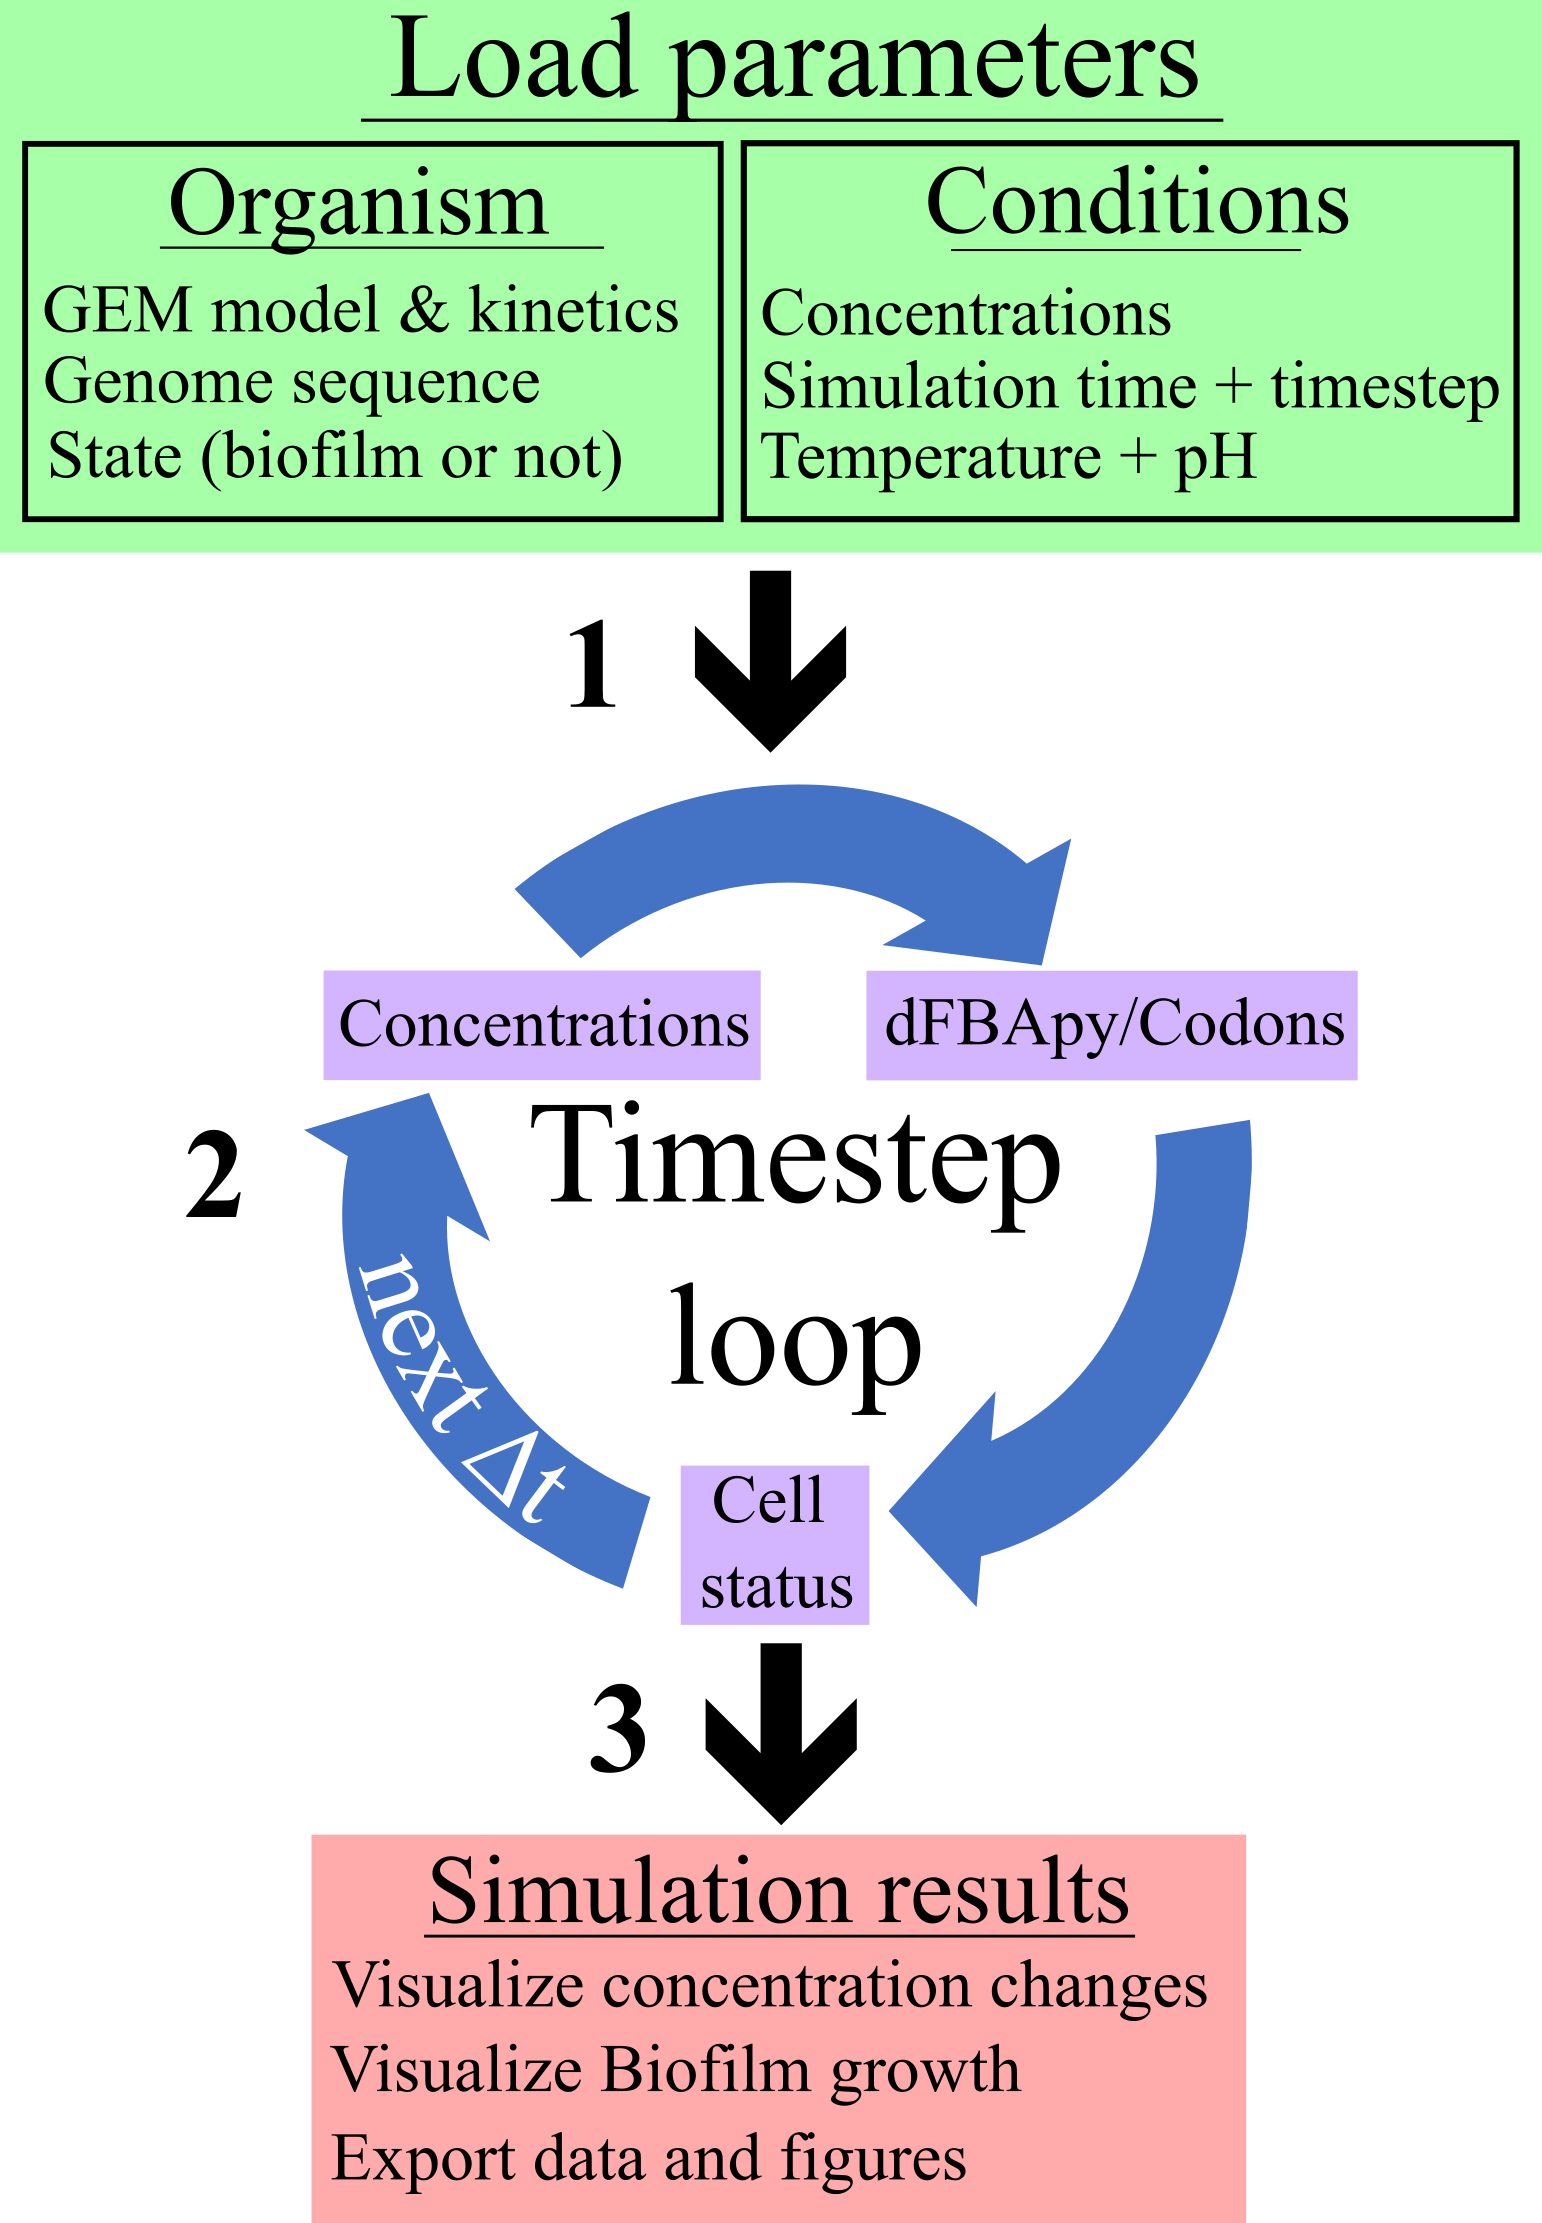
\includegraphics{images/wcmpy_workflow.png}
    \caption{
        The stepwise workflow of WCMpy. \textbf{Step 1} describes parameterizing the WCMpy simulation with information about the organism (i.e. the GEM model of metabolism and the corresponding kinetics rate laws, the genome sequence of the organism, and the simulated bacterial state of either planktonic or sessile) and the simulation conditions (i.e. the initial concentrations of the cytoplasm and the environment, the total simulated time and the timestep, and the temperature and pH of the system). \textbf{Step 2} describes the loop that occurs with each timestep: a) dFBA and the central dogma are conducted based upon previous concentrations; b) the cellular status and the mass/volume are calculated; and c) the concentrations are updated for the next timestep. \textbf{Step 3} describes processing, visualizing, and exporting the simulation results. 
    }
    \label{wcmpy_workflow}
\end{figure}

\section{Case studies}
We exemplify core functionality of the WCMpy workflow -- being the BiGG\_SABIO, dFBApy, and Codons modules -- in the following sections, which are available as Python Notebooks in the respective GitHub repositories.

\subsection{BiGG\_SABIO \& dFBApy}
The BiGG \textit{E. coli} core model consists only of the $95$ essential metabolic reactions for \textit{E. coli}. This model was first loaded into the BiGG\_SABIO module, where the \pyobject{parse\_data} function systematically acquired all of the data ($\approx 185 MB$) that describes the reactions of this model. The \pyobject{to\_fba} function then refined the raw data into a manageable file of kinetics data that was then directly parameterized into dFBApy and executed for an arbitrary amount of time. The results of this simulation are illustrated in Figure \ref{dfba}a, where the metabolic system re-establishes an equilibrium after the metabolism is perturbed by initial concentrations and rate law fluxes. The plotted concentrations for chemicals with defined initial concentrations are absolute concentrations, while those for chemicals without initial concentrations are only relative concentrations to the unknown initial concentration and are tagged with "(rel)" in the legend. The ability to alternatively parameterize kinetics data as an argument to the \pyobject{simulate} dFBApy function was demonstrated in Figure \ref{dfba}b by specifying only Acetate Kinase kinetic information from the full kinetic file of Figure \ref{dfba}a. 

\begin{figure}
    \centering
    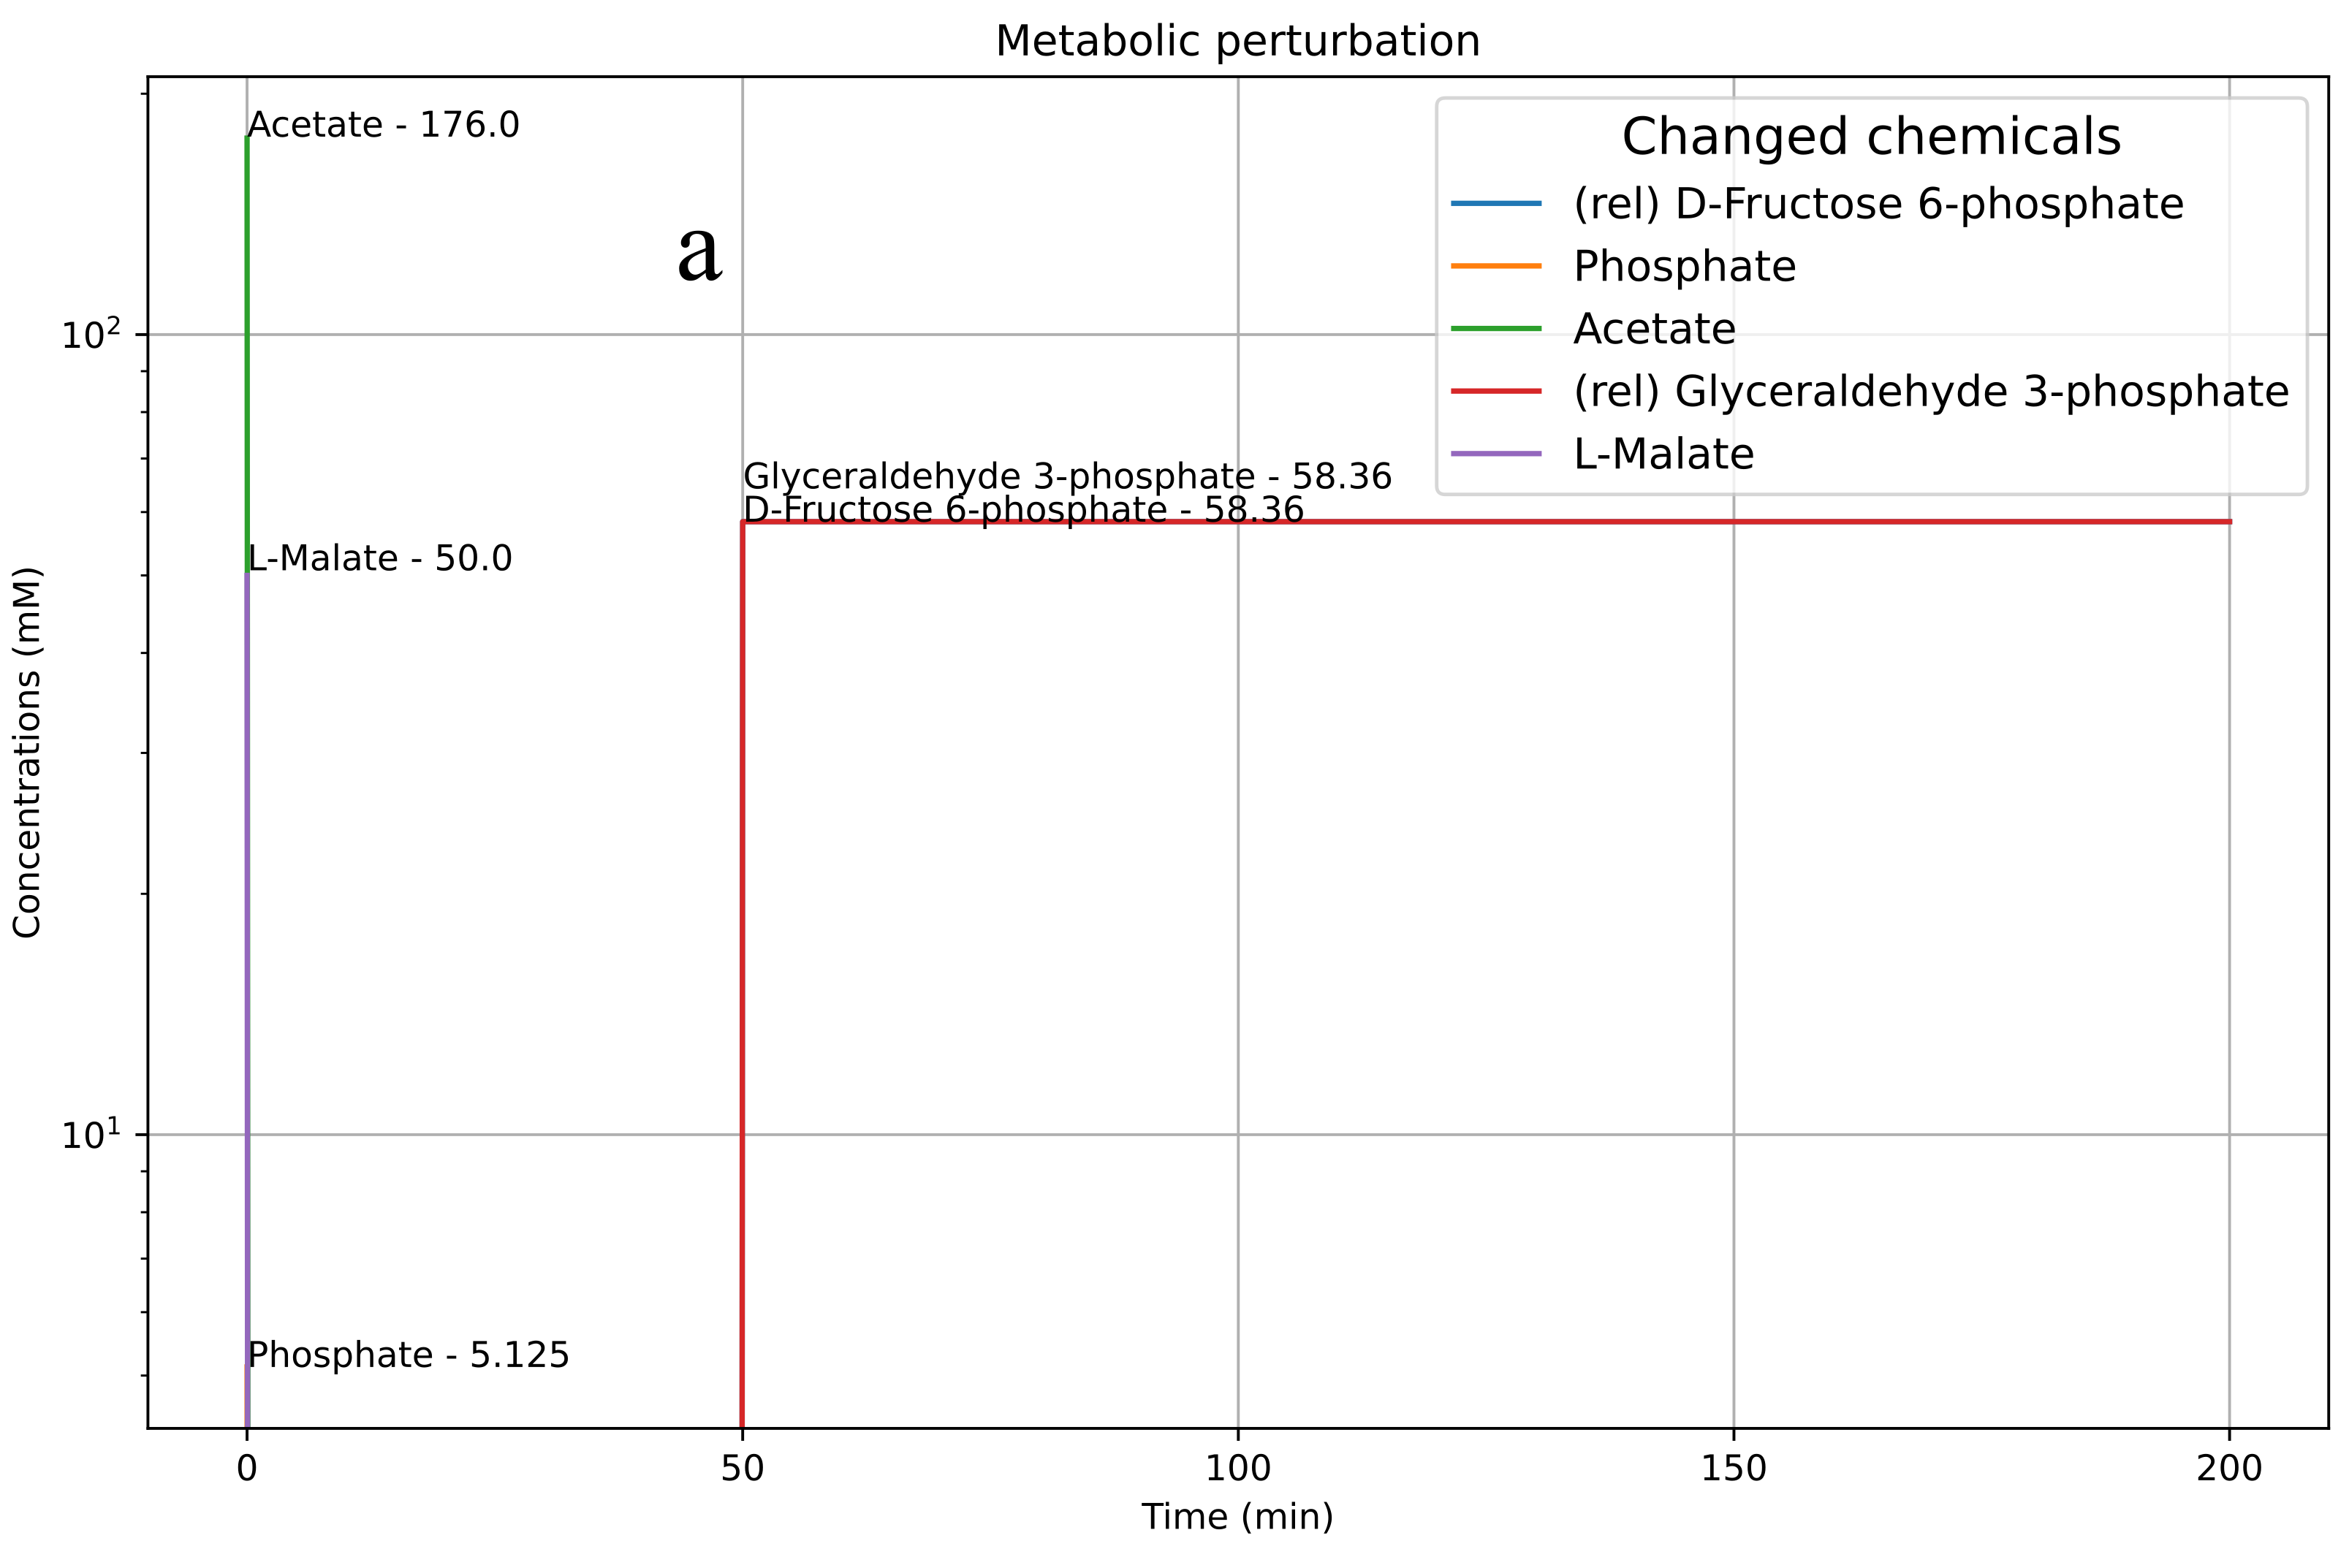
\includegraphics[width = 0.9\textwidth]{images/SABIO_dfba.png} \\
    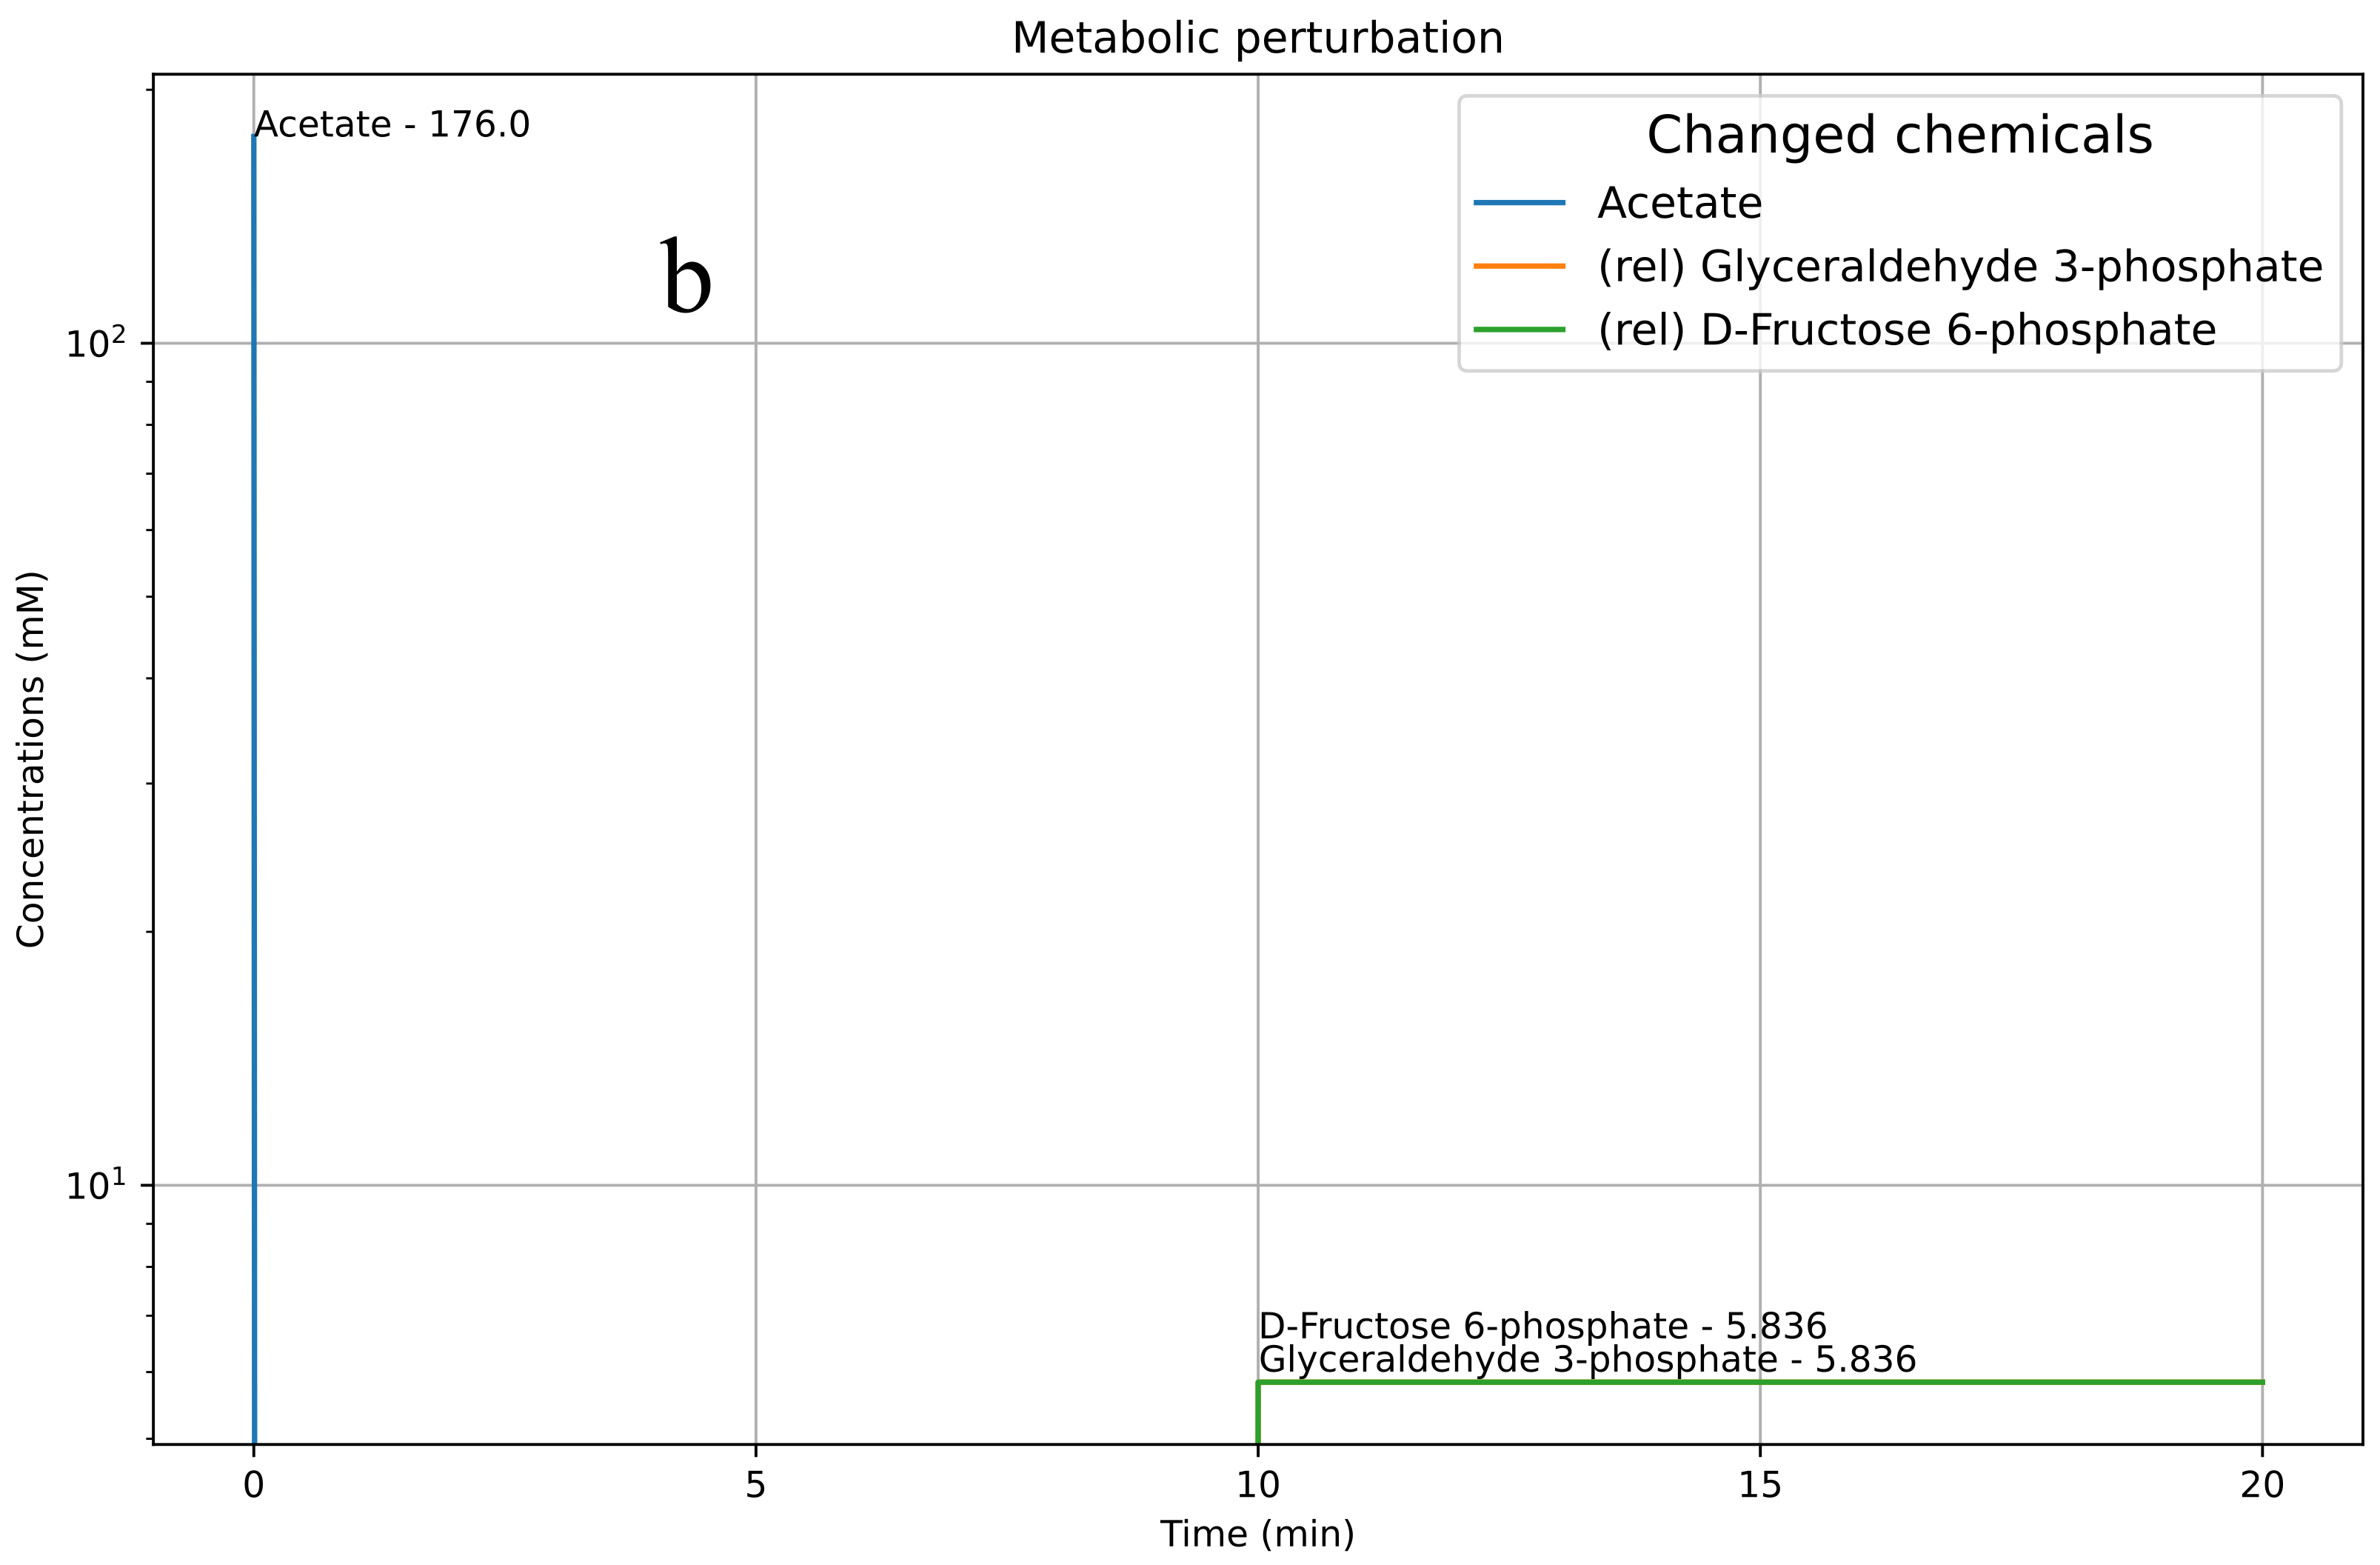
\includegraphics[width = 0.9\textwidth]{images/simple_argument.png}
    \caption{
        Notable concentration changes from dFBApy simulations of the \textit{E. coli} core BiGG model with a) SABIO-RK kinetics data via the BiGG\_SABIO module and b) a single entry from the kinetics data of a) that was passed as an argument in the API. The chemicals with non-zero concentration at time zero were defined with initial concentrations. The metabolic consequences of these concentrations and calculated fluxes are observed over the first timestep, where re-establishing equilibrium generates D-Xylulose 5-phosphate and Alpha-D-Ribose 5 phosphate with the carbon input. The concentrations of the generated metabolites are relative "(rel)" since their initial concentrations were not defined.
    }
    \label{dfba}
\end{figure}

\subsection{Codons}
The $\approx 29kb$ genetic sequence of the MERS (Middle-Eastern Respiratory Syndrome) virus was acquired from a published study \cite{Enouf2013MiddleGenome} that is organized within the NCBI BLASTn database. This genome was first searched in BLAST through Codons, and was independently identified to reflect the MERS virus, according to a multitude of cited studies. The sequence was then transcribed and translated in $70~ms$, and the resultant genetic and protein sequences were converted and exported as FASTA files. The 30 translated proteins were compared with the reported proteins for this BLAST entry of MERS that we sought to replicate, where approximately half of the predicted proteins matched perfectly with reported proteins and 96.5\% of the predicted peptide sequences were identified in the reported proteins. The deviations from 100\% are believed to result from peptide assembly into larger macromolecules and from viral-specific codon translations that were not implemented in the simulation. The translated proteins were finally searched in the BLAST database through Codons, where the largest proteins were identified with 100\% certainty while the ambiguity of small polypeptides was difficult for the database to identify. The rapid execution time and the high alignment of the predicted and reported peptides, nevertheless, support that the Codons module is a practical tool for emulating the central dogma. 

\section{Discussion}
The discrete steps in the metabolic plots of Figure \ref{dfba} are counter-intuitive, where continuous plots of concentration changes would be expected. This discrete behavior may be the consequence of the kinetic constraints being insufficiently time-dependent, although, the rate laws appear to possess the proper units and thus are generating fluxes with appropriate time dependency. The qualitative simularity and quantitative difference in the generated metabolites between Figures \ref{dfba}a-b, however, are both expected, since they simulate the same metabolic system and since the magnitude of generated metabolites is proportional to the carbon input from the initial concentrations, respectively. This supports that the module is consistent between simulations and reveals some expected behavior.

The WCMpy suite of Python packages contributes modular tools that we postulate will cultivate the development of a scalable WCM for molecularly resolved biofilm studies: WCMpy. The open-source network of Python encourages community efforts and will be particularly valuable for the development of a comprehensive project like WCMpy. The metabolome modules -- BiGG\_SABIO and dFBApy -- provide a novel conduit between kinetics databases and dFBA metabolic simulations for any organism whose metabolism is encapsulated in a BiGG-formatted GEM. These metabolic modules may, moreover, be individually useful to the DataNator \cite{Roth2021Datanator:Behavior} and ModelSEED \cite{Seaver2021TheMicrobes} projects that are developing bioinformatics and modelling tools, respectively, for applications in WCMs. The Codons module offers an intuitive and concise resource for simulating the central dogma of biology and investigating the genome and proteome of any organism with a known genetic sequence. These modules, collectively, mark a profound step towards alleviating the noted bottlenecks -- scalable code and bioinformatic logistics -- that hinder integrating biofilm models with fundamental WCMs towards facilitating biofilm research. 

\section{Author Contributions}
\begin{enumerate}
    \item \textbf{APF} - Writing and research
    \item \textbf{ESC} - Writing and research
    \item \textbf{HLB} - Writing, guidance, and funding
\end{enumerate}

\section{Acknowledgments}
The authors thank Jonathan R. Karr for his pioneering work in developing WCMs, and for providing guidance through our journey in systems biology.

% \setlength{\unitlength}{\savedunitlength}
